\label{Figure BoundingBoxConversion}
\begin{figure}[H]
    \centering
    \begin{center}
        $<label>\;<xCenterScaled>\;<yCenterScaled>\;<widthScaled>\;<heightScaled>$
    \end{center}
    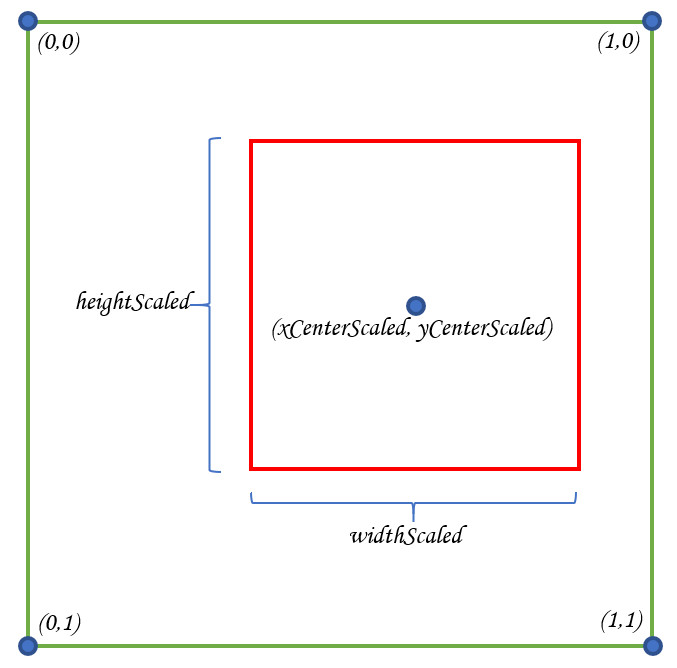
\includegraphics[width=0.5\textwidth]{images/boundingbox/BoundingBox-YOLO.jpg}
    \caption{YOLOv5 Pytorch label format}
    \label{fig:yolov5format}
\end{figure}

\begin{figure}[H]
    \centering
    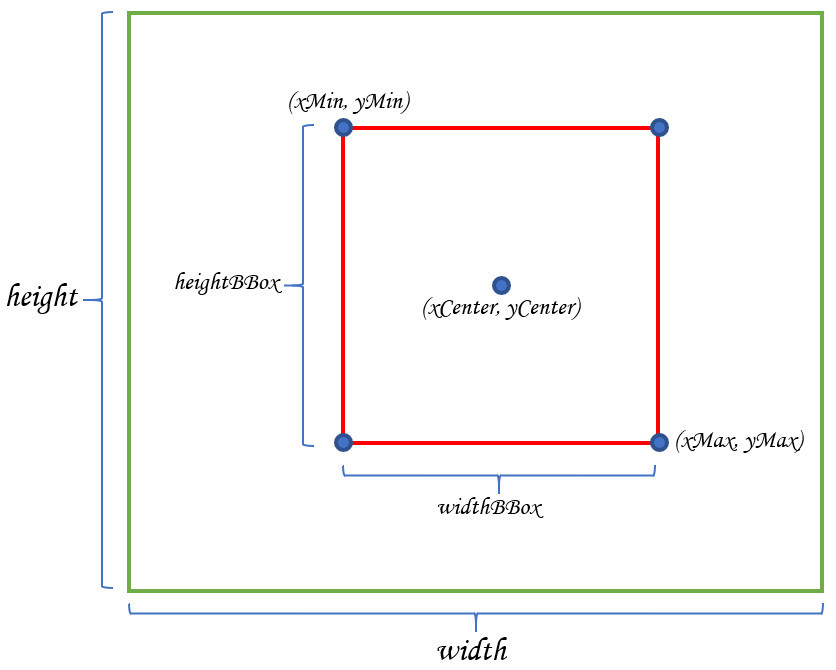
\includegraphics[width=0.7\textwidth]{images/boundingbox/BoundingBox-PascalVOC-COCO.jpg}
    \caption{Pascal VOC / COCO label format}
    \label{fig:otherformats}
\end{figure}
\clearpage

\begin{figure}[H]
    \begin{equation*}
        \begin{subfig}
            \begin{gathered}
                From\;Pascal\;VOC\;format \\
                xCenterScaled = \frac{\frac{xMin + xMax}{2} - 1}{width} \\
                yCenterScaled = \frac{\frac{yMin + yMax}{2} - 1}{height} \\
                widthScaled = \frac{xMax - xMin}{width} \\
                heightScaled = \frac{yMax - yMin}{height} \\
            \end{gathered}\hspace{6em}
        \end{subfig}
        \begin{subfig}
            \begin{gathered}
                From\;COCO\;format \\
                xCenterScaled = \frac{2 * xMin + widthBBox}{2 * width} \\
                yCenterScaled = \frac{2 * yMin + heightBBox}{2 * height} \\
                widthScaled = \frac{widthBBox}{width} \\
                heightScaled = \frac{heightBBox}{height} \\
            \end{gathered}
        \end{subfig}
    \end{equation*}
    \caption{Formulas to convert from other formats to YOLOv5 Pytorch format}
    \label{fig:conversionformula}
\end{figure}

\begin{figure}[H]
    \begin{align*}
        &xMin =\left\{\begin{matrix}
        0 \; if\; [(xCenterScaled - \frac{widthScaled}{2})*width] < 0 \\
        int([(xCenterScaled - \frac{widthScaled}{2})*width])+1 \; else,  \\
        \end{matrix}\right.\\
        &xMax =\left\{\begin{matrix}
        0 \; if\; [(xCenterScaled + \frac{widthScaled}{2})*width] > (width-1) \\
        int([(xCenterScaled + \frac{widthScaled}{2})*width])+1 \; else,  \\
        \end{matrix}\right. \\
        &yMin =\left\{\begin{matrix}
        0 \; if\; (yCenterScaled - \frac{heightScaled}{2})*height  \\
        int([(yCenterScaled - \frac{heightScaled}{2})*height])+1 \; else,  \\
        \end{matrix}\right.\\ 
        &yMax =\left\{\begin{matrix}
        height -1 \; if\; (yCenterScaled + \frac{heightScaled}{2})*height > (height-1) \\
        int([(yCenterScaled + \frac{heightScaled}{2})*height])+1 \; else,  \\
        \end{matrix}\right. 
    \end{align*}
    \caption{Formulas to convert from YOLOv5 Pytorch to Pascal VOC format}
    \label{fig:conversionformul}
\end{figure}

\begin{figure}[H]
    \centering
    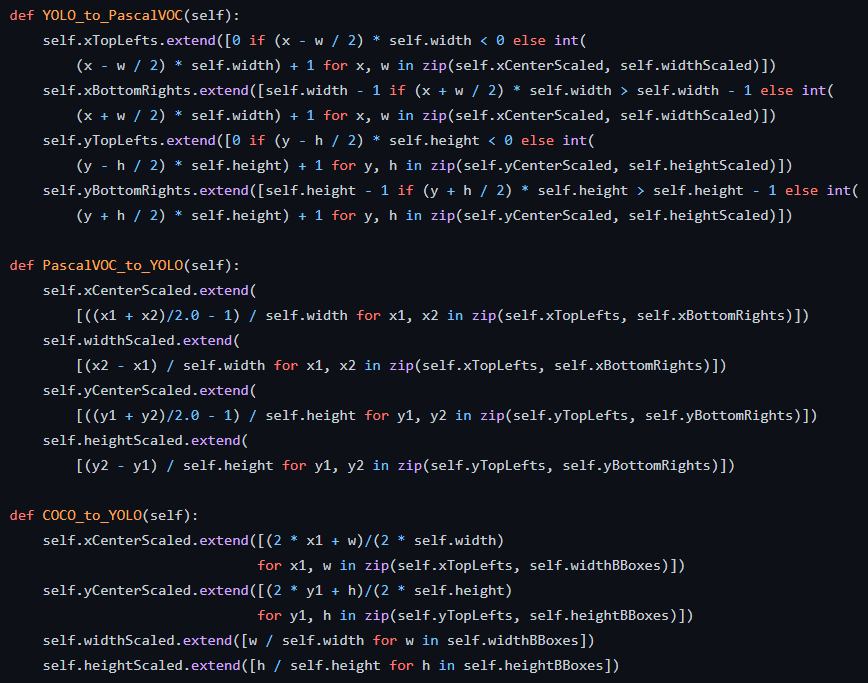
\includegraphics[width=0.75\textwidth]{images/boundingbox/CodeForBoundingBoxConversion.png}
    \caption{Code for Bounding Box Conversion}
    \label{fig:thefillerarc}
\end{figure}